\chapter{Estudio de bases de datos} \label{ch:databases-study}

La selección de datos para la implementación del segmentador se extrajo de \textsc{PhysioNet}, organización apoyada
por \textit{National Institute of General Medical Sciences} (\acrshort{nigms}) y \textit{National Institute of
Biomedical Imaging and Bioengineering} (\acrshort{nibib}). Esta organización se dedica a ofrecer, de manera
gratuita, acceso a un gran cantidad de señales fisiológicas y herramientas para el procesamiento de las mismas. \\
\indent Particularmente, se extrajeron dos base de datos. Una asociada a a un desafío público en el año 2016 que se
denominaba ``\textit{Classification of Normal/Abnormal Heart Sound Recordings: the PhysioNet/Computing in Cardiology
Challenge 2016}``, el cual consistía en diseñar e implementar un clasificador de fonocardiogramas normales y
anormales bajo ciertas condiciones. En el Cuadro \ref{tab:challenge2016} se mencionan las características generales
de la base de datos.

\begin{table}[H]
  \centering
  \begin{tabular}{ |c|c|c|c|c|c|c| }
    \hline
    \thead{Set} & \thead{Cantidad \\ de archivos} & \thead{Normal} & \thead{Anormal} & \thead{Duración \\
    promedio [s]} & \thead{Máx. \\ dureación [s]} & \thead{Mín. \\ duración [s]} \\
    \hline
    \thead{training-a} & \thead{409} & \thead{117} & \thead{292} & \thead{32.56} & \thead{36.5} & \thead{9.27} \\
    \thead{training-b} & \thead{490} & \thead{386} & \thead{104} & \thead{7.98} & \thead{8} & \thead{5.31} \\
    \thead{training-c} & \thead{31} & \thead{7} & \thead{24} & \thead{49.44} & \thead{122} & \thead{9.65} \\
    \thead{training-d} & \thead{55} & \thead{27} & \thead{28} & \thead{15.15} & \thead{48.54} & \thead{6.61} \\
    \thead{training-e} & \thead{2141} & \thead{1958} & \thead{183} & \thead{23.07} & \thead{101.67} & \thead{8.06} \\
    \thead{training-f} & \thead{114} & \thead{34} & \thead{114} & \thead{33.12} & \thead{59.62} & \thead{29.38} \\
    \hline
  \end{tabular}
  \caption[Base de datos: Challenge 2016]{Base de datos: Challenge 2016. Tipos y características de los sonidos
  cardíacos.}
  \label{tab:challenge2016}
\end{table}

\indent Señales recolectadas en ambientes clínicos y no clínicos, y de pacientes sanos y patológicos. El total es de
3126 fonocardiogramas para el set de entrenamiento (sólo el set A viene acompañado de señales del \acrshort{ecg} y
300 fonocardiogramas para el set de validación. \\
\indent Estos fonocardiogramas fueron extraídos del área aórtica, área pulmonar, área tricúspide y mitral. En cada
subset de datos, se clasificaron en fonocardiogramas normales y anormales. Los fonocardiogramas normales fueron
extraídos de pacientes sanos y los anormales de pacientes con problemas cardíacos. Los pacientes sufren de distintas
enfermedades cardíacas que no se encuentran detalladas en cada uno de los pacientes. Sin embargo, las enfermedades
cardíacas típicas son deficiencias valvulares y enfermedades asociadas a las coronarias. Las deficiencias valvulares
incluyen prolapso de la válvula mitral, regurgitación mitral, estenosis aórtica y cirugías valvulares. Todos los
pacientes sanos y patológicos incluyen adultos y niños, y cada uno de éstos pueden aportar de uno a seis grabaciones
. Adicionalmente, cada una de las grabaciones fue muestreada a 2000 Hz y una única derivación del fonocardiograma. \\
\indent Es importante tener en cuenta, dado a que las grabaciones fueron hechas en ambientes no controlados, muchas
de éstas se encuentan contaminadas por diferentes fuentes de ruido, como el habla, movimiento del estetoscopio,
respiración y ruidos intestinales. \\
\indent La segunda base de datos ha sido publicada por David Springer a partir del trabajo en \cite{pp:springer2015}
. Si bien no es exactamente la base de datos utilizada en su trabajo, fue aportada por él junto a una implementación
hecha en \textsc{MATLAB\texttrademark}. \\
\indent A diferencia de la base del \textit{Challenge 2016}, posee 792 grabaciones de fonocardiogramas muestreadas a
una frecuencia de 1000 Hz. Éstas fueron extraídas de 135 pacientes, y más de una grabación por paciente. También, se
han dividido grabaciones en varias secciones por inconsistencias de anotaciones. \\
\indent Las anotaciones están basadas en electrocardiogramas (no presentes en el set de datos), las cuales
involucran la onda R y el fin de la onda T muestreadas a 50 Hz. Estas anotaciones fueron extraídas de manera
automática mediante un método de concordancia, el cual se detallará en la Sección \ref{sec:annotations}. \\
\indent Por otro lado, se utilizó una clasificación binaria para definir cada grabación como patológica o no
patológica.

\section{Selección y normalización de datos} \label{sec:data-selection-normalization}

Ya vimos que estas base de datos contienen datos que difieren entre si. Desde la cantidad de señales hasta los tipos
de datos (\acrshort{ecg}, anotaciones del \acrshort{ecg}, frecuencia de muestreo). \\
\indent Dicho esto es necesario decidir por una base de datos en una primera instancia. Para ponerlo en términos
cuantitativos, por qué la elección de una base respecto de la otra, se menciona lo siguiente. La frecuencia de
muestreo no es un problema, por lo tanto tanto 1 KHz como 2 KHz es más que suficiente para tener una buena
resolución en tiempo. Ambas bases clasifican las señales respecto a si son patológicas o no patológicas, es decir,
que es posible realizar algún tipo de entrenamiento para la clasificación de éstas, aunque no es el alcance de este
trabajo y no afecta a la selección de los datos. Sin embargo, esto sirve para identificar que la base no se
encuentre desbalanceada respecto a la proporción de sanos como enfermos. El punto crítico de la selección de la base
se debe a las anotaciones del electocardiograma. La base de datos de Springer \cite{ref:logi-regression-springer} ya
contiene marcas extraídas automáticamente y filtradas por un algoritmo de concordancia. De lo contrario, en la base
de datos del desafío se proveen los \acrshort{ecg}, a los cuales es necesario extraerles las marcas correspondientes.
Debido a que el alcance del trabajo es implementar un segmentador de PCG y no un extractor de anotaciones, se optó
por utilizar la base de David Springer dado a que permite apoyarse sobre trabajos previos que ya han utilizado
dichos datos, confiando en la naturaleza de estos datos y así realizar una mejor comparación en el Capítulo
\ref{ch:results}. Asimismo, se referirá a la base seleccionada como \textit{base de datos} para evitar confusión. \\
\indent Los datos de la base de datos se encuentran en formato \texttt{.mat} (formato propietario de
\textsc{MATLAB\texttrademark}) y las anotaciones de las ondas R y fin de la T, se encuentran muestreadas a 50 Hz.
Esto requiere de estandarizar el formato de los datos y acomodar la frecuencia de las anotaciones dado a que las
señales se encuentran a una frecuencia de muestreo mayor. Para ello, se tomó como estándar el formato
\acrshort{wfdb} (\textit{Waveform Database}), el cual contiene dos categorías estándar, \textit{MIT Format} y
\textit{EDF Format}.

\subsection*{MIT Format}
\begin{itemize}
  \item Los archivos \textit{MIT Signal} (\texttt{.dat}) son archivos binarios que contienen muestras de señales
  digitalizadas. Éstas almacenan las señales, pero no pueden ser interpretados sin los \textit{header} files.
  Los archivos son de la forma: \texttt{\{RECORD\_NAME\}.dat}.
  \item Los archivos \textit{MIT Header} (\texttt{.hea}) son archivos de texto cortos que describen el contenido
  del archivo de la señal asociado.
  \item Los archivos \textit{MIT Annotation} son archivos binarios que contienen anotaciones (etiquetas que
  generalmente refieren a muestras específicas de una señal asociada). Éstos deben ser leídos junto a los archivos
  \textit{header} asociado. En caso de que en un directorio se vean archivos \texttt{\{RECORD\_NAME\}.dat}, y/o
  \texttt{\{RECORD\_NAME\}.hea}, cualquier otro archivo con otra extensión es un archivo de anotaciones. Por ejemplo,
  \item \texttt{\{RECORD\_NAME\}.atr} es un archivo con anotaciones para esa señal.
\end{itemize}

\subsection*{EDF Format}
\begin{itemize}
  \item Los archivos \href{http://www.edfplus.info/specs/edf.html}{\underline{EDF}} contienen señales digitalizadas
  \item almacenadads en formato internacional. Estos archivos guardan la información de encabezado al comienzo del
  \item archivo, a diferencia del formato MIT. A su vez pueden estar acompañados de archivos con anotaciones.
  \item Por ejemplo, si existe un archivo \texttt{*.edf}, un archivo con anotaciones asociado podría ser
  \item \texttt{*.edf.qrs}, donde \texttt{.qrs} es la extensión de las anotaciones en este caso (podría ser otro).
  \item Los archivos
  \href{http://www.edfplus.info/specs/edfplus.html}{\underline{EDF+}} son archivos EDF que contienen anotaciones
  \item codificadas como señales.
\end{itemize}

\indent La categoría utilizada en este trabajo es \textit{MIT Format}. Este formato debe ser leído con una librería
especializada. \textit{WFDB Software Package} es un conjunto de funciones para escribir y leer en formatos
específicos de \textit{PhysioBank databases} (entre otros). La librería \textit{WFDB} es \textit{LGPLed}, y puede
ser usada para programas escritos en \textit{ANSI/ISO C}, \textit{K\&R C}, \textit{C++}, o \textit{Fortran},
corriendo bajo sistemas operativos para los cuales el compilador \textit{ANSI/ISO} or \textit{K\&R C} se encuentre
disponible, incluyendo todas las versiones Unix, MS-DOS, MS-Windows, the Macintosh OS, y VMS. Opcionalmente, la
librería de WFDB puede ser compilada con HTTP o FTP como input sin tener que bajar localmente toda la base de datos
para un procesamiento. \\
\indent En este trabajo se utilizó \textit{WFDB Toolbox for MATLAB\texttrademark}, el cual provee acceso desde
\textsc{MATLAB\texttrademark} a las aplicaciones de \texttt{WFDB}. Esta toolbox provee \textsc{MATLAB\texttrademark} y
Java
\textit{wrappers} para las distintas aplicaciones y un instalador que instala la toolbox en sí misma y el
\textit{WFDB Software Package} precompilado. Esta toolbox corre en 64-bit \textsc{MATLAB\texttrademark} R2010b o
mayor en \textit{GNU/Linux}, \textit{Mac OS X}, y \textit{MS-Windows}. \\
\indent El set de datos de Springer, fue convertido de \textit{MAT Format} a \textit{MIT Format}, donde el
directorio tiene la estructura de la Figura \ref{fig:springer-db}. Los archivos \texttt{.dat} contienen la señal del
PCG. La información ejemplo de los archivos \texttt{.hea} se observan en la Figura \ref{fig:hea-info} y los archivos
\texttt{.ann} contienen las anotaciones de las ondas R y el fin de la T, de acuerdo al estándar provisto por
\textsc{PhysioNet}.

\begin{figure}[H]
  \centering
  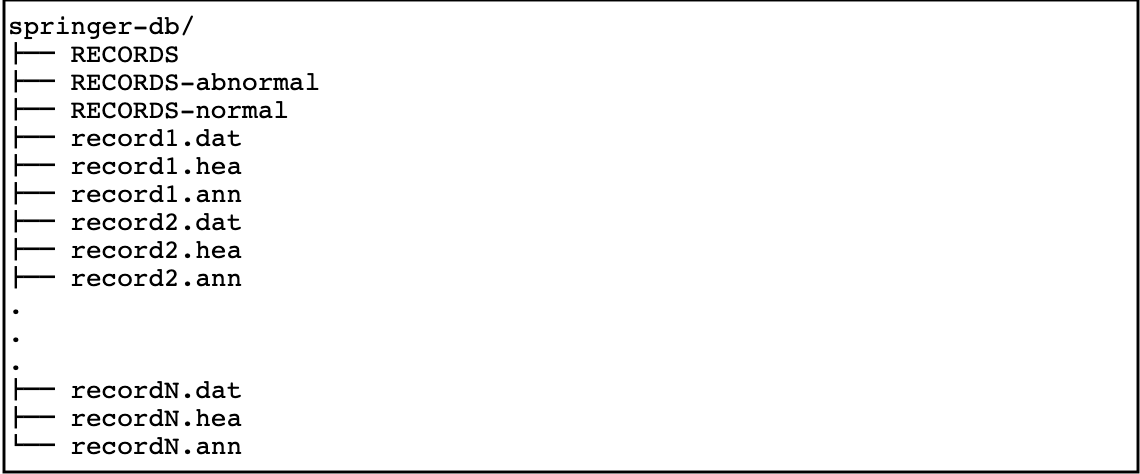
\includegraphics[scale=0.73]{sections/chapter-03/images/springer-db.png}
  \caption[Estructura del directorio de la base de datos.]{Estructura del directorio de la base de datos. El
  archivo \texttt{RECORDS} contiene en un archivo de texto los nombres de la señales del set de datos, lo mismo
  para \texttt{RECORDS-abnormal} y \texttt{RECORDS-normal}, asociados a señales patológicas y no patológicas
  respectivamente.}.
  \label{fig:springer-db}
\end{figure}

\begin{figure}[H]
  \centering
  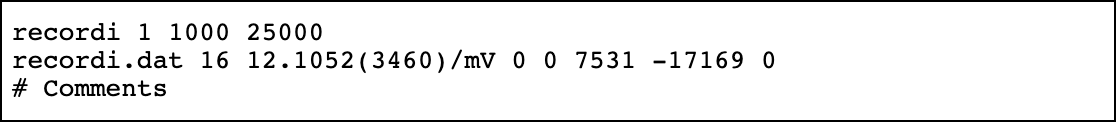
\includegraphics[scale=0.74]{sections/chapter-03/images/hea-info.png}
  \caption[Información ejemplo del archivo header de una señal]{Información ejemplo del archivo header de una
  señal. En la primer línea se encuentra, de forma ordenada, el nombre de la señal, la cantidad de señales en el
  archivo \texttt{.dat}, la frecuencia de muestreo en Hz y la cantidad de muestras. La segunda línea contiene el
  nombre del archivo y a continuacíon información de adquisción.}
  \label{fig:hea-info}
\end{figure}

\indent En cuanto a la corrección de las anotaciones provistas en la base de datos que se encuentran submuestreadas
a 50 Hz. Para ello, se recupera la frecuencia original a partir de la ecuación \ref{eq:adapt-annotations}.

\begin{align}
  \label{eq:adapt-annotations}
  \bm{a}_{f_2} = \frac{f_2}{f_1} \cdot \bm{a}_{f_1}
\end{align}

\indent Donde $f_1 = 50$ Hz y $f_2 = 1000$ Hz.
